\section* {4.1 Методы Эйлера, Рунге-Кутты и Адамса}

\subsection{Постановка задачи}
Реализовать методы Эйлера, Рунге-Кутты и Адамса 4-го порядка в виде программ, задавая в качестве входных данных шаг сетки  . С использованием разработанного программного обеспечения решить задачу Коши для ОДУ 2-го порядка на указанном отрезке. Оценить погрешность численного решения с использованием метода Рунге – Ромберга и путем сравнения с точным решением. 

\subsection{Вариант: 28}
Задача Коши:{x^2 * y'' + 3*x*y' +4*y -5*x = 0, y(1)=6, y'(1)=8, для x от 1 до 2 с шагом h=0.1}, 
$ y=5*x + x^2 + x^2 * ln|x|
% \pagebreak

\subsection{Результаты работы}
\begin{figure}[h!]
\centering
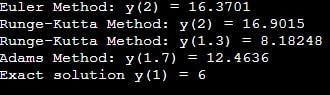
\includegraphics[width=15cm, height=7.5cm]{img/img1.jpg}
\caption{Вывод программы в консоли}
\end{figure}

\pagebreak

\subsection{Исходный код}

\lstinputlisting{include/task_1.cpp}
\pagebreak

\section* {4.2 Метод стрельбы и конечно-разностный метод}

\subsection{Постановка задачи}
Реализовать метод стрельбы и конечно-разностный метод решения краевой задачи для ОДУ в виде программ. С использованием разработанного программного обеспечения решить краевую задачу для обыкновенного дифференциального уравнения 2-го порядка на указанном отрезке. Оценить погрешность численного решения с использованием метода Рунге – Ромберга и путем сравнения с точным решением. 

{\bfseries Вариант:} 28

Краевая задача:{x*y'' - (2*x + 1)*y' +2y=0, y'(0)=2, y(1)=exp(x)}, y=exp(2*x)
% \pagebreak

\subsection{Результаты работы}
\begin{figure}[h!]
\centering
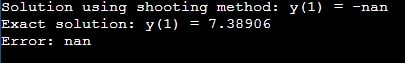
\includegraphics[width=.9\textwidth]{img/img2.jpg}
\caption{Вывод программы в консоли}
\end{figure}

\pagebreak

\subsection{Исходный код}

\lstinputlisting{include/task_2.cpp}
